\documentclass[10pt,a4paper]{scrartcl}
\usepackage[utf8]{inputenc}
\usepackage[T1]{fontenc}
\usepackage[ngerman]{babel}
\usepackage{microtype, multicol, marginnote, bera, parskip}
\usepackage{listings, amsmath, amssymb, graphicx, tikz, epic}
\usepackage{stmaryrd} %for lightning arrow
\usepackage{pstricks, pst-node, pst-tree, pdflscape}
\usepackage[babel=true]{csquotes}
\usepackage{placeins}
\tolerance=2000
\setcounter{secnumdepth}{0}
\usepackage[inner=2cm,outer=2cm,top=1.5cm,bottom=1.5cm,includeheadfoot]{geometry}
\newcommand{\subExercise}[1]{\vspace{0.5em} \noindent{\bf #1)}}
\author{Michael Mardaus \and Andrey Tyukin}
\title{
\includegraphics[scale=0.2]{../logo_schriftzug}\\
Technische Informatik: Abgabe 4}

\begin{document}

\maketitle

\section*{Exercise 4.1 (Full adder from decoder)}

\vspace{1em}
\begin{figure}[h]
  \centering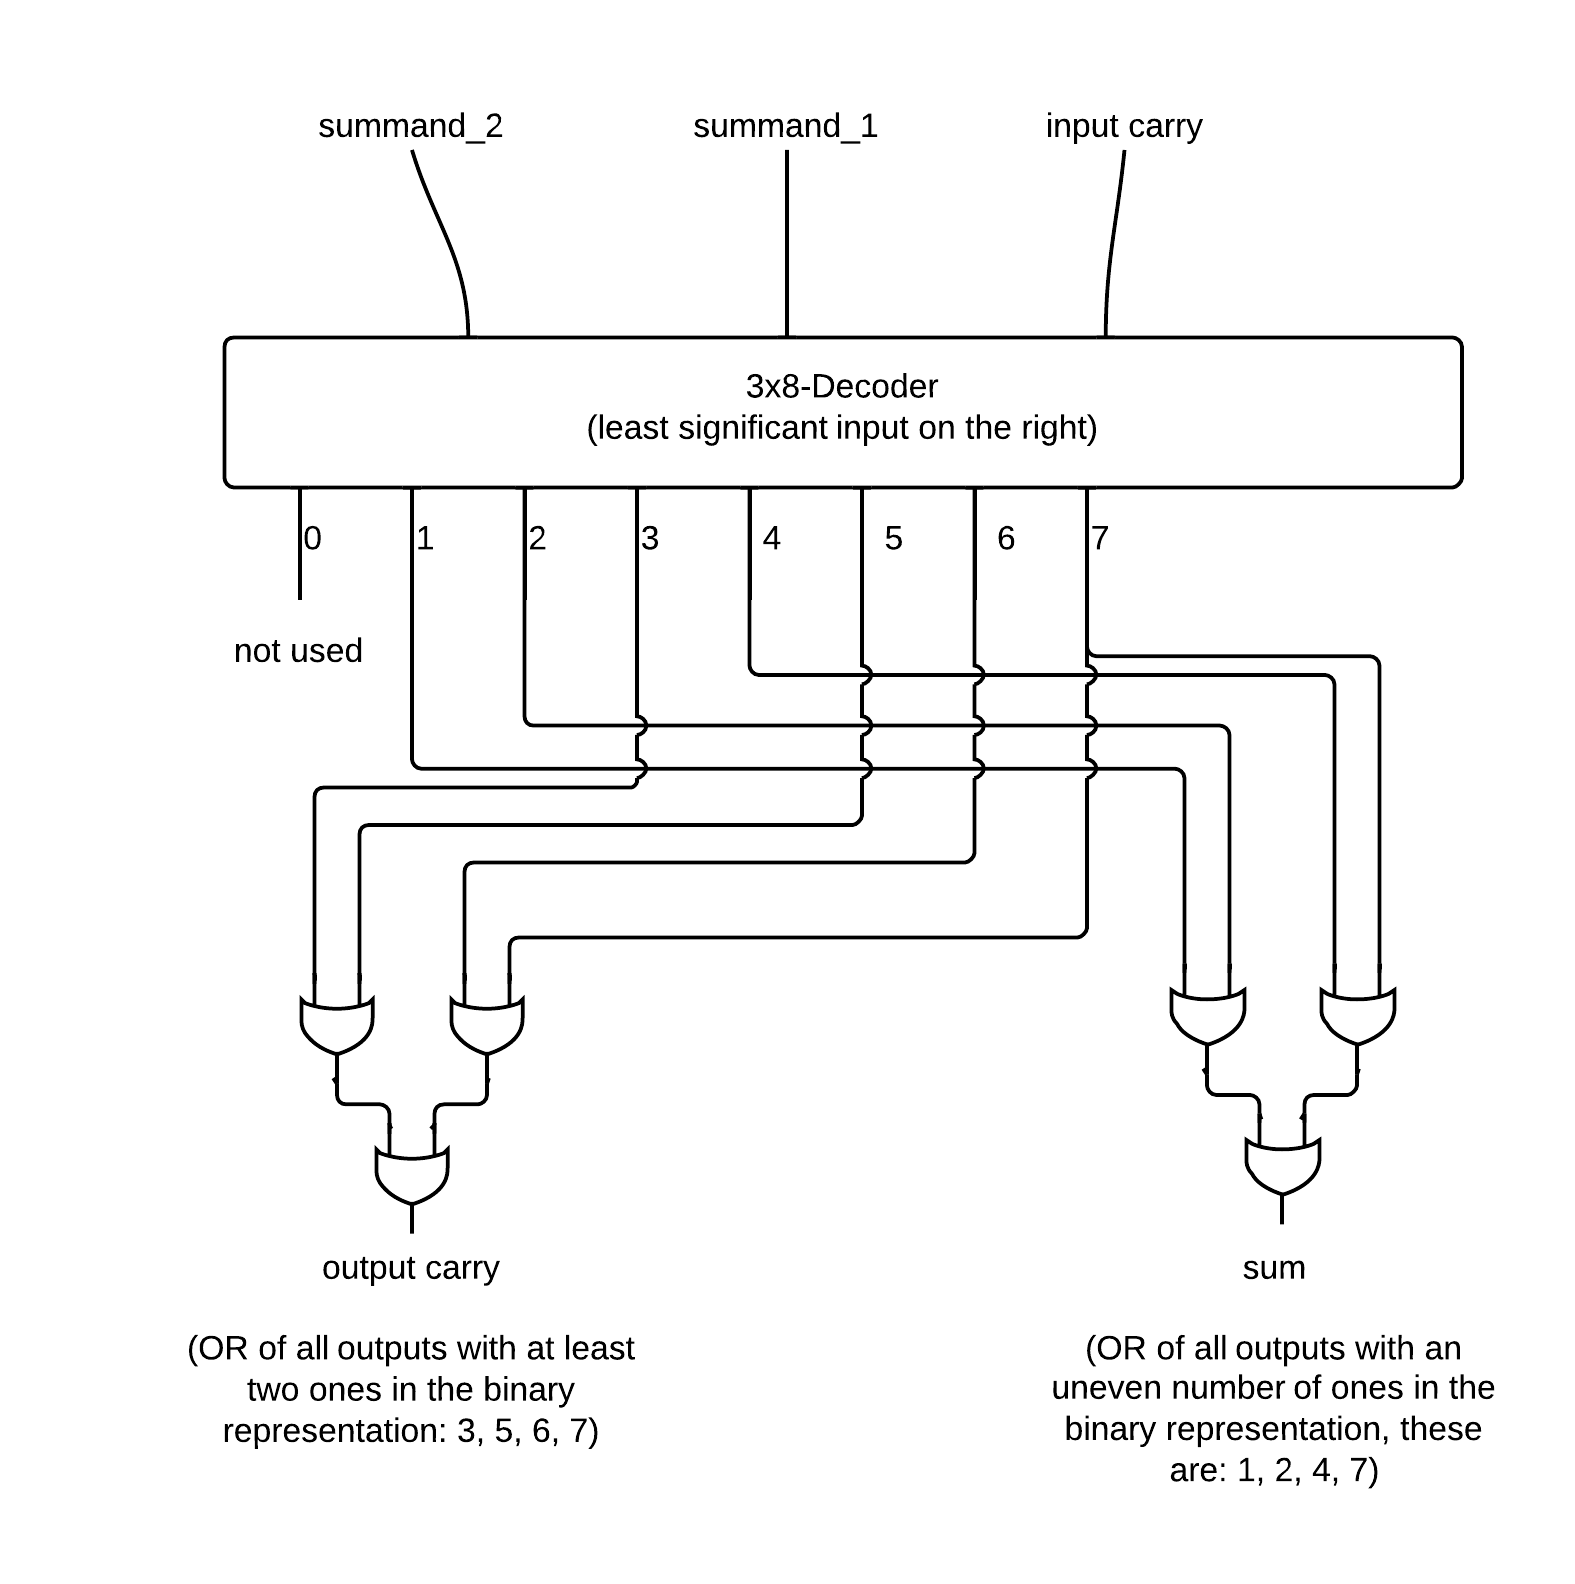
\includegraphics[width=0.6\linewidth]{images/fullAdder.png}
\end{figure}
\vspace{1em}

\FloatBarrier
\newpage
\section*{Exercise 4.2 (TODO)}
\subExercise{a}
\subExercise{b}
\subExercise{c}
\subExercise{d}

\section*{Exercise 4.3 (TODO)}
\subExercise{a}
\subExercise{b}

\end{document}
